%%%%%%%%%%%%%%%%%%%%%%%%%%%%%%%%%%%%%%%%%
% Beamer Presentation
% LaTeX Template
% Version 1.0 (10/11/12)
%
% This template has been downloaded from:
% http://www.LaTeXTemplates.com
%
% License:
% CC BY-NC-SA 3.0 (http://creativecommons.org/licenses/by-nc-sa/3.0/)
%
%%%%%%%%%%%%%%%%%%%%%%%%%%%%%%%%%%%%%%%%%

%----------------------------------------------------------------------------------------
%	PACKAGES AND THEMES
%----------------------------------------------------------------------------------------

\documentclass{beamer}

\mode<presentation> {

% The Beamer class comes with a number of default slide themes
% which change the colors and layouts of slides. Below this is a list
% of all the themes, uncomment each in turn to see what they look like.

%\usetheme{default}
%\usetheme{AnnArbor}
%\usetheme{Antibes}
%\usetheme{Bergen}
%\usetheme{Berkeley}
%\usetheme{Berlin}
%\usetheme{Boadilla}
%\usetheme{CambridgeUS}
%\usetheme{Copenhagen}
%\usetheme{Darmstadt}
%\usetheme{Dresden}
%\usetheme{Frankfurt}
%\usetheme{Goettingen}
%\usetheme{Hannover}
%\usetheme{Ilmenau}
%\usetheme{JuanLesPins}
%\usetheme{Luebeck}
\usetheme{Madrid}
%\usetheme{Malmoe}
%\usetheme{Marburg}
%\usetheme{Montpellier}
%\usetheme{PaloAlto}
%\usetheme{Pittsburgh}
%\usetheme{Rochester}
%\usetheme{Singapore}
%\usetheme{Szeged}
%\usetheme{Warsaw}

% As well as themes, the Beamer class has a number of color themes
% for any slide theme. Uncomment each of these in turn to see how it
% changes the colors of your current slide theme.

%\usecolortheme{albatross}
%\usecolortheme{beaver}
%\usecolortheme{beetle}
%\usecolortheme{crane}
%\usecolortheme{dolphin}
%\usecolortheme{dove}
%\usecolortheme{fly}
%\usecolortheme{lily}
%\usecolortheme{orchid}
%\usecolortheme{rose}
%\usecolortheme{seagull}
%\usecolortheme{seahorse}
%\usecolortheme{whale}
%\usecolortheme{wolverine}

%\setbeamertemplate{footline} % To remove the footer line in all slides uncomment this line
%\setbeamertemplate{footline}[page number] % To replace the footer line in all slides with a simple slide count uncomment this line

%\setbeamertemplate{navigation symbols}{} % To remove the navigation symbols from the bottom of all slides uncomment this line
}

\usepackage[utf8]{inputenc}
\usepackage{ragged2e}
\usepackage[export]{adjustbox}
\usepackage[flushleft]{threeparttable}
\usepackage{graphicx} % Allows including images
\usepackage{booktabs} % Allows the use of \toprule, \midrule and \bottomrule in tables
\usepackage[portuguese]{babel}
\usepackage{adjustbox}
\usepackage{graphicx}
\usepackage{multicol}

%----------------------------------------------------------------------------------------
%	TITLE PAGE
%----------------------------------------------------------------------------------------

\title[Exame de Qualificação]{Caracterização de eventos de exceção e de seus respectivos impactos no sistema de transporte público por ônibus da cidade de São Paulo} % The short title appears at the bottom of every slide, the full title is only on the title page

\author[DIAS, F.; CORDEIRO, D.]{Felipe Cordeiro Alves Dias\\[1mm]Orientador: Prof. Dr. Daniel de Angelis Cordeiro}
\institute[USP-EACH] % Your institution as it will appear on the bottom of every slide, may be shorthand to save space
{
Universidade de São Paulo \\ % Your institution for the title page
\medskip
}
\date{\today} % Date, can be changed to a custom date

\begin{document}

\begin{frame}
\titlepage % Print the title page as the first slide
\end{frame}
%----------------------------------------------------------------------------------------
%	PRESENTATION SLIDES
%----------------------------------------------------------------------------------------

%------------------------------------------------
\section{Introdução}
\begin{frame}
\Huge{\centerline{Introdução}}
\end{frame}
%------------------------------------------------
\subsection{Motivação}
\begin{frame}
\frametitle{Motivação}
\begin{itemize}
\item Segregação urbana: dentre os mais de 12 milhões de habitantes da cidade de São Paulo, 10\% estão localizados no Centro Expandido (CE) e 90\% no Cinturão Periférico (CP).
\begin{itemize}
\item Movimento pendular e (CP) como região dormitória.
\item Problemas relacionados a mobilidade urbana.
\end{itemize}
\end{itemize}

\begin{itemize}
\item Legislação federal e municipal sobre mobilidade urbana.
\begin{itemize}
\item Lei Federal 12.587/2012: para desenvolvimento sustentável com a mitigação dos custos ambientais e socioeconômicos dos deslocamentos de pessoas.
\item Decreto 56.834: institui o \textit{PlanMob/SP 2015} como instrumento de planejamento e gestão do Sistema Municipal de Mobilidade Urbana para os próximos 15 anos.
\end{itemize}
\end{itemize}

\end{frame}

%------------------------------------------------
\begin{frame}
\frametitle{Motivação}
\begin{itemize}
\item \textit{PlanMob/SP 2015}
\begin{itemize}
\item Criação da Central Integrada de Mobilidade Urbana (CIMU): com o objetivo de integrar as áreas de trânsito e transporte subordinadas à Secretaria Municipal de Transportes (SMT).
\item A CIMU não processa conteúdo de Redes Sociais;
\item não aborda melhorias dos sistemas já existentes;
\item será integrada com o desfasado SIM.
\end{itemize}
\end{itemize}

\begin{itemize}
\item Sistema Integrado de Monitoramento e Transporte (SIM): localização e rastreio dos ônibus, fornece informações em tempo real aos passageiros, monitora 1.353 rotas de ônibus, 10 corredores de ônibus, 28 terminais de ônibus e 19.933 mil paradas de ônibus que serviram em 2016 a aproximadamente 8 milhões de passageiros por dia. \item Apesar da importância do SIM, há inúmeras defasagens tecnológicas (que causam discrepância nas informações recebidas pelos usuários, dentre outros problemas).
\end{itemize}
\end{frame}
%------------------------------------------------
\begin{frame}
\frametitle{Motivação}
\begin{itemize}
\item Sistemas de Transporte Inteligente (ITS --- \textit{Intelligent Transport System}).
\item A lei de mobilidade urbana (12.587/2012) e o \textit{PlanMob/SP 2015} não mencionam explicitamente ITS e TIC.
\item O transporte público pode se beneficiar ao explorar ITS, e ao integrar as Redes Sociais com o planejamento, gestão e as atividades operacionais dos transportes públicos, abordando seus respectivos fatores sócio-técnicos.
\item Analisar o impacto dos eventos de exceção na operação do sistema de transporte público por ônibus na cidade de São Paulo, usando dados do SIM (AVL) e de Redes Sociais.
\end{itemize}
\end{frame}
%------------------------------------------------
\subsection{Definição do problema}
\begin{frame}
\frametitle{Definição do problema}
\begin{itemize}
\item Eventos de exceção: acidentes, greves, falhas na operação do metrô, manifestações, enchentes, eventos sociais, dentre outros.
\end{itemize}

\begin{itemize}
\item Identificação de características dos eventos de exceção.
\begin{itemize}
\item Dados históricos dos módulos AVL do SIM.
\begin{itemize}
\item Processamento de grandes volumes de dados;
\item qualidade dos dados comprometida.
\end{itemize}
\item Twitter.
\begin{itemize}
\item Identificação dos eventos de exceção nas publicações; 
\item geolocalizá-los; 
\item extração e identificação de \textit{timestamps};
\item correlacioná-los com a base histórica.
\end{itemize}
\end{itemize}
\end{itemize}

\begin{itemize}
\item Uso de tais características para análise, aprendizado e simulação de como os eventos de exceção impactam o transporte público por ônibus.
\end{itemize}

\end{frame}
%------------------------------------------------
\subsection{Objetivos}
\begin{frame}
\frametitle{Objetivos}
\begin{block}{Gerais}
Caracterização de eventos de exceção e de seus respectivos impactos no sistema de transporte público por ônibus da cidade de São Paulo.
\begin{itemize}
\item \textbf{Observação}: Com a utilização de \textit{tweets} das contas oficiais das instituições responsáveis por reportar eventos de exceção na cidade de São Paulo e dados históricos dos módulos AVL do SIM.
\end{itemize}
\end{block}
\end{frame}
%------------------------------------------------
\begin{frame}
\frametitle{Objetivos}
\begin{table}[!htb]
\centering
\caption{Descrição e nome dos profiles selecionados do Twitter}
	\label{tab:oficialProfiles}
\begin{adjustbox}{max height=28mm}
\begin{threeparttable}
\begin{tabular}{c|c}
\hline
\textbf{Descrição do \textit{profile} no \textit{Twitter}} & \textbf {Profile no \textit{Twitter}} \\ 
\hline
Comando do Corpo de Bombeiros da PMESP \tnote{a} & \textit{@BombeirosPMESP} \\ 
\hline
Companhia de Engenharia de Tráfego de SP & \textit{@CETSP\_} \\ 
\hline
Companhia Paulista de Trens Metropolitanos & \textit{@CPTM\_oficial} \\ 
\hline
Defesa Civil do Estado de São Paulo & \textit{@SPCEDEC} \\
\hline
Governo do Estado de São Paulo & \textit{@governosp} \\
\hline
Metrô de São Paulo & \textit{@metrosp\_oficial} \\
\hline
Polícia Cívil do Estado de São Paulo & \textit{@Policia\_Civil} \\  
\hline
Polícia Militar do Estado de São Paulo & \textit{@PMESP} \\ 
\hline
São Paulo Agora --- CCOI \tnote{b} & \textit{@saopaulo\_agora} \\
\hline
São Paulo Transporte & \textit{@sptrans\_} \\
\hline
São Paulo Turismo & \textit{@TurismoSaoPaulo} \\ 
\hline
Secretaria de Transportes de São Paulo & \textit{@smtsp\_} \\ 
\hline
\end{tabular}
\begin{tablenotes}
            \item[a] Polícia Militar do Estado de São Paulo.
            \item[b] Centro de Controle Integrado 24 Horas da Cidade de São Paulo
        \end{tablenotes}
\end{threeparttable}
\end{adjustbox}
\end{table}
\end{frame}
%------------------------------------------------
\begin{frame}
\frametitle{Objetivos}
\begin{block}{Específicos}
\begin{itemize}
    \item Identificar os eventos de exceção, quando existentes, dos \textit{tweets} coletados.
     \item Extrair os endereços dos eventos de exceção identificados e geolocalizá-los.
		\item Construir uma base de dados pública com os dados processados, disponibilizada via API (para consumo e contribuição da comunidade de software), mantendo o modelo de dados consistente.
\item Criação de plataforma para exploração e visualização dos dados coletados e processados das fontes citadas na Tab. \ref{tab:oficialProfiles} e da SPTrans.
\end{itemize}
\end{block}
\end{frame}
%------------------------------------------------
\subsection{Hipóteses}
\begin{frame}
\frametitle{Hipóteses}
Com base na Revisão Sistemática realizada, os eventos de exceção presentes nos \textit{tweets} podem ser caracterizados, não exaustivamente, em:

\begin{itemize}
\item \textbf{Acidentes}.
\begin{itemize}
\item Acidentes nas estações de transporte.
\item Incêndio.
\end{itemize}

\item \textbf{Espaço-temporais}.
\begin{itemize}
\item Dia da semana.
\item Hora do dia.
\end{itemize}

\item \textbf{Eventos sociais}.
\begin{itemize}
\item Feiras de rua.
\item Festivais.
\item Jogos esportivos.
\item Passeatas e maratonas.
\end{itemize}

\item \textbf{Eventos urbanos}.
\begin{itemize}
\item Relacionados ao tráfego.
\end{itemize}

\end{itemize}

\end{frame}
%------------------------------------------------
\begin{frame}
\frametitle{Hipóteses}

\begin{itemize}
\item \textbf{Desastres naturais}.
\begin{itemize}
\item Tempestades.
\item Terremoto.
\item Tufões.
\end{itemize}

\item \textbf{Metereológicas}.
\begin{itemize}
\item Dia claro, nublado, chuvoso, nevando, com neblina.
\item Temperatura do ar.
\end{itemize}
\end{itemize}

\begin{itemize}

\item Identificação de características utilizando Processamento de Linguagem Natural (NLP --- \textit{Natural Language Processing}) em conjunto com dicionários auxiliares para o contexto dos eventos de exceção mencionados.

\item Extração dos endereços dos \textit{tweets} utilizando a técnica de Expressão Regular e posterior geolocalização.
\end{itemize}

\end{frame}
%------------------------------------------------
\section{Fundamentação Teórica}
\begin{frame}
\Huge{\centerline{Fundamentação Teórica}}
\end{frame}
%------------------------------------------------
\subsection{Cidades Inteligentes}
\begin{frame}
\frametitle{Cidades Inteligentes}
\begin{block}{Cidades Inteligentes (SC --- \textit{Smart Cities})}
São cidades sustentáveis e socialmente inclusivas, que utilizam Tecnologias da Informação e Comunicação (TICs) para gerir eficientemente seus respectivos recursos naturais.
\begin{itemize}
\item \textit{TDM --- Technology Driven Method; top-down}; de fornecimento.
\item \textit{HDM --- Human Driven Method; bottom-up}; de demanda.
\end{itemize}
\end{block}

\begin{block}{Cidade}
Complexo e dinâmico sistema sócio-técnico. Composto por sistemas urbanos, com espaços físicos para a vida cotidiana e com sistemas de infraestrutura.
\end{block}
\end{frame}
%------------------------------------------------
\begin{frame}
\frametitle{Cidades Inteligentes}
\begin{itemize}
\item As TICs permeiam os sistemas urbanos e espaços físicos: dados voluntários, de sensores e Redes Sociais.
\item Desafios relacionados a conectividade:
\begin{itemize}
\item Infraestrutura de rede.
\item interoperabilidade;
\item padrões;
\item consumo de energia;
\item escalabilidade, dentre outros.
\end{itemize}
\item Desafios relacionados aos dados:
\begin{itemize}
\item Capacidade e local de armazenamento;
\item extração;
\item tratamento;
\item processamento;
\item análise;
\item integração;
\item agregação de dados, dentre outros.
\end{itemize}
\end{itemize}
\end{frame}
%------------------------------------------------
\subsection{Sistemas de Transporte Inteligente}
\begin{frame}
\frametitle{Sistemas de Transporte Inteligente}
\begin{block}{Sistemas de Transporte Inteligentes (ITS --- \textit{Intelligent Transportation Systems})}
Tem como fim utilizar TICs para resolver problemas relacionados ao transporte, tais como congestionamento, segurança, eficiência e conservação ambiental. 
\end{block}
\begin{itemize}
\item \textbf{\textit{Advanced Traffic Management System} (ATMS)} --- são sistemas utilizados para melhorar a qualidade do serviço de tráfego e redução de atrasos.
\item \textbf{\textit{Advanced Travellers Information Systems} (ATIS)} --- são sistemas utilizados para fornecer informação em tempo real aos viajantes.
\end{itemize}

\end{frame}
%------------------------------------------------
\begin{frame}
\frametitle{Sistemas de Transporte Inteligente}
\begin{itemize}
\item  \textbf{\textit{Advanced Public Transportations Systems} (APTS)} --- são sistemas que utilizam ATMS e ATIS para melhorar a eficiência e operação do transporte público coletivo.
\item \textbf{\textit{Advanced Vehicles Control Systems} (AVCS)} --- são sistemas compostos por sensores, computadores e sistemas de controle para auxiliar e alertar motoristas, com o objetivo de melhorar a segurança e reduzir congestionamentos.
\item \textbf{\textit{Commercial Vehicles Operation} (CVO)} --- são sistemas utilizados para a segurança de veículos comerciais e frotas, por meio de tecnologias relacionadas a gerenciamento de tráfego, controle e gerenciamento de veículos e informações aos viajantes, tais como:
\begin{itemize}
\item \textit{Automatic Vehicles Identification}.
\item \textit{Automatic Vehicles Classification}.
\item \textit{\textbf{Automatic Vehicles Location}}.
\item \textit{Pedestrian Movement Detection}.
\item \textit{Board Computers}.
\item \textit{Real Time Traffic Transmissions}.
\end{itemize}
\end{itemize}
\end{frame}
%------------------------------------------------
\subsection{Conceitos relacionados ao transporte público}
\begin{frame}
\frametitle{Conceitos relacionados ao transporte público}
\begin{itemize}
\item Acessibilidade.
\item Acessibilidade universal.
\item Mobilidade.
\item Mobilidade urbana.
\begin{itemize}
\item Transporte público coletivo;
\item  transporte de alta capacidade;
\item  acessibilidade universal nos passeios e edificações;
\item prioridade ao transporte coletivo no sistema viário;
\item terminais de transporte intermodais;
\item rede de transporte coletivo por ônibus (com acessibilidade universal);
\item rede cicloviária;
\item bicicletários e paraciclos;
\item  legibilidade dos sistemas de orientação;
\item comunicação eficaz com os usuários;
\item modicidade tarifária;
\item  logística eficiente no transporte de carga, dentre outros itens.
\end{itemize} 
\end{itemize}
\end{frame}
%------------------------------------------------
\subsection{General Transit Feed Specification}
\begin{frame}
\frametitle{General Transit Feed Specification}
\begin{block}{\textit{GTFS --- General Transit Feed Specification}}
É uma especificação de um formato comum para troca de informações estáticas sobre transporte público. Um \textit{feed} especificado na GTFS estática é composto por arquivos de texto que modelam diferentes perspectivas do transporte público, tais como paradas, trajetos, viagens e outros dados relativos a horário.
\end{block}
\begin{itemize}
\item {\textit{GTFS-realtime}}.
\begin{itemize}
\item Atualizações dos horários de parada: viagem programada, adicionada, cancelada, desprogramada, cancelada, substituição e indefinição.
\item Alertas de serviço: frequência, entidades afetadas, causa e efeito (sem serviço, serviço reduzido, atrasos significativos, desvio, serviço adicional, serviço modificado, parada deslocada, outro efeito, efeito desconhecido).
\item Posições de veículos: posição, nível de congestionamento e estado de parada do veículo.
\end{itemize}
\end{itemize}
\end{frame}
%------------------------------------------------
\begin{frame}
\frametitle{General Transit Feed Specification}
Arquivos obrigatórios da GTFS:
\begin{itemize}
\item \textit{agency.txt}: agências de transporte público como fonte de dados.
\item \textit{stops.txt}: locais de embarque e desembarque.
\item \textit{routes.txt}: trajetos de um grupo de viagens.
\item \textit{trips.txt}: viagens de cada trajeto.
\item \textit{stop\_times.txt}: horários de partida e chegada em paradas.
\item \textit{calendar.txt}: início, fim e dias disponíveis dos serviços.
\end{itemize}
\end{frame}
%------------------------------------------------
\subsection{Redes Sociais}
\begin{frame}
\frametitle{Redes Sociais}
\begin{block}{Redes Sociais}
As Redes Sociais podem ser definidas como redes que possuem muitos relacionamentos, com grandes componentes conectados, altos coeficientes de agrupamento e grau de reciprocidade. Ex.: Facebook.
\end{block}
\begin{block}{Rede de Informações}
Nesse tipo de rede a interação dominante é a disseminação de informações entre os relacionamentos, com baixo baixo índice de reciprocidade. Ex.: Twitter.
\end{block}
\end{frame}
%------------------------------------------------
\subsection{Processamento de Linguagem Natural}
\begin{frame}
\frametitle{Processamento de Linguagem Natural}
\begin{block}{{Processamento de Linguagem Natural}}
Explora como computadores podem ser utilizados para entender e manipular texto ou fala em linguagem natural, o que envolve conhecimento interdisciplinar principalmente entre as áreas de ciência da computação, linguística e estatística.
\end{block}
\begin{multicols}{2}
\begin{itemize}
\item Problemas de baixo nível (comuns a NLP).
\begin{itemize}
\item \textit{Sentence boundary disambiguation};
\item \textit{Tokenization};
\item \textit{Part-of-speech tagging};
\item dentre outros.
\end{itemize}
\end{itemize}

\columnbreak

\begin{itemize}
\item Problemas de alto nível (específicos e com base nos problema de baixo nível).
\begin{itemize}
\item \textit{Spelling / grammatical error identification and recovery};
\item \textit{Named Entity Recognition};
\item \textit{Word Sense Disambiguation};
\item dentre outros.
\end{itemize}
\end{itemize}
\end{multicols}
\end{frame}
%------------------------------------------------
\subsection{Feature Engineering}
\begin{frame}
\frametitle{Feature Engineering}
\begin{block}{Feature Engineering}
Processo iterativo de construção, extração e seleção de características (features), o qual depende do conhecimento de domínio e de suas respectivas métricas.
\end{block}
\begin{itemize}
\item Características (\textit{features}) binárias, categóricas ou contínuas.
\item Pré-processamento: técnicas de padronização, normalização, remoção de ruídos, redução de dimensionalidade, discretização, expansão, etc.
\end{itemize}
\end{frame}
%------------------------------------------------
\subsection{Algorítimos de Aprendizado de Máquina}
\begin{frame}
\frametitle {Algorítimos de Aprendizado de Máquina}
\begin{itemize}
\item Supervisionados;
\begin{itemize}
\item \textit{Artificial Neural Network};
\item \textit{Decision Tree};
\item \textit{Decision Rules Classification};
\item \textit{K-nearest neighbor (k-NN)};
\item \textit{Fuzzy correlation};
\item \textit{Genetic Algorithm};
\item \textit{Naïve Bayes Algorithm};
\item \textit{Rocchio's Algorithm};
\item \textit{Support Vector Machine}.
\end{itemize}
\item não-supervisionados;
\item semi-supervisionados;
\item por reforço.
\end{itemize}
\end{frame}
%------------------------------------------------
\section{Revisão Sistemática}
\begin{frame}
\Huge{\centerline{Revisão Sistemática}}
\end{frame}
%------------------------------------------------
\begin{frame}
\frametitle{Revisão Sistemática}
\begin{block}{Quais os tipos de problemas urbanos abordados utilizando processamentos de \textit{tweets}? (QP1)}
\begin{itemize}
\item \textit{e-Participation}.
\item Detecção de zoneamento urbano.
\item Identificação de pontos de interesse.
\item Mobilidade.
\item Padrões demográficos.
\item Poluição.
\item Segurança Pública.
\item Turismo.
\item Tráfego.
\end{itemize}
\end{block}
\end{frame}
%------------------------------------------------
\begin{frame}
\frametitle{Revisão Sistemática}
\begin{block}{Casos de uso relacionados ao transporte público (QP2)}
\begin{itemize}
\item Impacto de eventos no transporte público.
\begin{itemize}
\item Impacto dos ataques terroristas em Paris no uso do transporte público.
\item Impacto de eventos relacionados ao tráfego na demanda por bicicletas, em Nova Iorque e Washington D.C, EUA.
\item Impacto dos pontos de interesse na demanda por transporte público.
\item Impacto dos eventos anormais nas tomadas de decisão dos passageiros do Metrô de Tokyo.
\item Predição de fluxo de passageiros no Metrô de Nova Iorque.
\end{itemize}

\item Planejamento e gestão do transporte público.
\begin{itemize}
\item Análise de sentimento relacionada ao acesso ao transporte público.
\item Coleta de informações relacionadas ao transporte público.
\item Identificação de locais para estações de bicicletas, em St. Petersburg, Rússia.
\item Identificação da disposição dos usuários para realizar viagens de lazer.
\item Plataforma para notificação de problemas relacionados ao transporte público de Bangalore, Índia.
\end{itemize}
\end{itemize}
\end{block}

\end{frame}
%------------------------------------------------
\begin{frame}
\frametitle{Revisão Sistemática}
\begin{block}{Técnicas estatísticas utilizadas no processamento de \textit{tweets} (QP3)}
\begin{itemize}
\item Análise de métricas relacionadas a desempenho.
\item \textit{Cosine similarity}.
\item \textit{${F_1}$ score}.
\item \textit{Term frequency–inverse document frequency} (TF-IDF).
\item \textit{Inverse coefficient of variation}.
\item \textit{Jackknife resampling}.
\item \textit{Linear Regression}.
\item \textit{Local Indicators of Spatial Association} (LISA).
\item \textit{Local Moran's}.
\item \textit{Maximum likelihood estimation}.
\item \textit{Seasonal Autoregressive Integrated Moving Average} (SARIMA).
\item \textit{Optimization and Prediction with hybrid loss function}.
\end{itemize}
\end{block}
\end{frame}
%------------------------------------------------
\begin{frame}
\frametitle{Revisão Sistemática}
\begin{block}{Paradigmas de processamento (QP4)}
\begin{itemize}
\item \textit{Batch processing} (offline).
\item \textit{Near Real Time}.
\item \textit{Real Time}.
\end{itemize}
\end{block}

\begin{block}{Eventos de exceção relacionados ao transporte público (QP5)}
\begin{itemize}
\item Acidentes.
\begin{itemize}
\item Acidentes nas estações transporte.
\item Incêndio.
\end{itemize}

\item Espaço-temporais.
\begin{itemize}
\item Dia da semana.
\item Hora do dia.
\end{itemize}

\end{itemize}
\end{block}

\end{frame}
%------------------------------------------------
\begin{frame}
\frametitle{Revisão Sistemática}
\begin{block}{Eventos de exceção relacionados ao transporte público (QP5)}
\begin{itemize}
\item Eventos sociais.
\begin{itemize}
\item Feiras de rua.
\item Festivais.
\item Jogos esportivos.
\item Passeatas e maratonas.
\end{itemize}

\item Eventos urbanos.
\begin{itemize}
\item Relacionados ao tráfego.
\end{itemize}

\item Desastres naturais.
\begin{itemize}
\item Tempestades.
\item Terremoto.
\item Tufões.
\end{itemize}

\item Metereológicas.
\begin{itemize}
\item Dia claro, nublado, chuvoso, nevando, com neblina.
\item Temperatura do ar.
\end{itemize}

\end{itemize}
\end{block}
\end{frame}
%------------------------------------------------
\begin{frame}
\frametitle{Revisão Sistemática}
\begin{block}{Técnicas de Aprendizado de Máquina utilizadas no processamento de \textit{tweets} (QP6)}
\begin{itemize}
\item \textit{Bayes classification}.
\item \textit{C5.0 algorithm}.
\item \textit{Conditional Random Field (CRF) with Logistic Regression}.
\item \textit{Event extraction based on tweet hashtags}.
\item \textit{Latent Dirichlet Allocation} (LDA).
\item \textit{Monte Carlo simulation}.
\item \textit{PairFac} (técnica inovadora que utiliza \textit{Tensor Factorization}).
\item \textit{Random Forest classification}.
\item \textit{Support Vector Machine}.
\item \textit{Self-Organizing Maps}.
\end{itemize}

\end{block}
\end{frame}
%------------------------------------------------
\section{Proposta de pesquisa}
\begin{frame}
\Huge{\centerline{Proposta de pesquisa}}
\end{frame}
%------------------------------------------------
\subsection{Formalização do problema}
\begin{frame}
\frametitle{Proposta de Pesquisa}
\begin{block}{Formalização do problema}
O problema de caracterização de eventos de exceção e de seus respectivos impactos envolve a fase conhecida como \textit{feature extraction}. \textit{Feature extraction} consiste na extração de um conjunto de características ${\alpha =}$ $\lbrace {\chi_1}, {\chi_2}, ..., {\chi_n} \rbrace$ a partir de um dado de entrada $\chi$. Sendo assim, nessa proposta de pesquisa pretendemos extrair o conjunto de características ${E = }$ $\lbrace {\varepsilon_1}, {\varepsilon_2}, ..., {\varepsilon_n} \rbrace$, referente a cada evento de exceção, e o conjunto ${I_{\varepsilon_i} = }$ $\lbrace {\iota_{1\varepsilon_i}}, {\iota_{2\varepsilon_i}}, ..., {\iota_{n\varepsilon_i}} \rbrace$, contendo as características de cada impacto decorrente de um determinado evento de exceção $\varepsilon_i \in E$. \newline \newline Tem-se também como problema a correlação de cada evento de exceção com o seu respectivo impacto, permitindo assim uma análise histórica para identificação de padrões de causa e consequência.
\begin{equation*} 
\forall \iota \in I, \exists \varepsilon \in E (\iota = f(\varepsilon) ) 
\end{equation*}
\end{block}
\end{frame}
%------------------------------------------------
\subsection{Solução proposta}
\begin{frame}
\frametitle{Proposta de pesquisa}
\begin{figure}
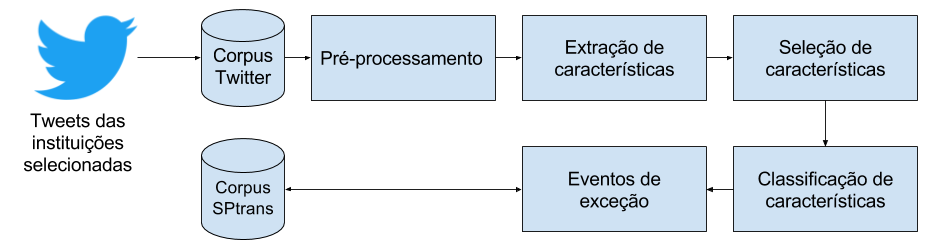
\includegraphics[width=1\linewidth]{solution}
\end{figure}
Expressão regular para extração de endereços:
\begin{equation}
ER = \lbrace L_1|S_1|L_2|S_2|...|L_n|S_n \rbrace \lbrace [a-zA-Z \backslash s]+ \rbrace
\end{equation}
Geolocalização dos endereços usando a API do Google Geocoding.
\end{frame}
%------------------------------------------------
\subsection{Construção do conjunto de dados}
\begin{frame}
\frametitle{Corpus Twitter}
\begin{table}[!htb]
\centering
\caption{Intervalo de tempo e número de \textit{tweets} coletados}
	\label{tab:tweetsCollected}
\begin{adjustbox}{max height=28mm}
\begin{threeparttable}
\begin{tabular}{c|c|c|c}
\hline
\textbf {Profile no \textit{Twitter}} &\textbf{ \# tweets \tnote{a}}  &\textbf{ \textit{Timestamp 1 \tnote{b}}} & \textbf{\textit{Timestamp 2 \tnote{c}}} \\ 
\hline
BombeirosPMESP & 5750 & 2017-05-21 02:10:39 & 2017-10-29 23:07:08  \\
\hline
CETSP\_ & 5042 & 2017-02-20 14:07:04 & 2017-10-29 21:45:54 \\ 
\hline
CPTM\_oficial & 5435 & 2017-04-24 13:00:17 & 2017-10-29 10:00:40 \\ 
\hline
governosp & 5450 & 2017-05-10 17:00:05 & 2017-10-29 22:00:03 \\
\hline
metrosp\_oficial & 7296 & 2017-06-07 17:23:34  & 2017-10-29 17:48:12 \\
\hline
Policia\_Civil & 3360 & 2015-04-15 17:44:44 & 2017-10-27 10:01:53 \\  
\hline
PMESP & 3956 & 2016-06-02 17:21:32 & 2017-10-29 20:25:37 \\ 
\hline
saopaulo\_agora & 3671 & 2016-11-18 07:36:12 & 2017-10-29 20:56:28 \\
\hline
smtsp\_ & 1128 & 2017-04-26 10:44:26 & 2017-10-29 23:00:11 \\ 
\hline
SPCEDEC & 945 & 2015-06-09 10:50:23 & 2017-10-29 23:38:36 \\
\hline
sptrans\_ & 8447 & 2017-06-13 15:19:56 & 2017-10-29 22:01:44 \\
\hline
TurismoSaoPaulo & 3308 & 2012-06-12 22:00:38 & 2017-10-27 17:46:59 \\ 
\hline
\hline
\textbf{Total} & 53788 & - & -   \\
\hline
\hline
\end{tabular}
\begin{tablenotes}
            \item[a] Número de \textit{tweets} coletados.
            \item[b] \textit{Timestamp} mais antigo.
            \item[c] \textit{Timestamp} mais recente.
        \end{tablenotes}
\end{threeparttable}
\end{adjustbox}
\end{table}
\end{frame}
%------------------------------------------------
\begin{frame}
\frametitle{Corpus SPTrans}
\begin{table}[!htb]
\centering
\caption{Conjuntos e quantidades de dados especificados em GTFS pela SPTrans}
	\label{tab:gtfs}
\begin{adjustbox}{max height=15mm}
\begin{tabular}{c|c}
\hline
\textbf{Conjunto de dados} & \textbf {Quantidade de dados} \\ 
\hline
\textit{agency.txt} & 1 \\ 
\hline
\textit{calendar.txt} & 6 \\ 
\hline
\textit{fare\_attributes.txt} & 6 \\ 
\hline
\textit{fare\_rules.txt} & 5.400 \\
\hline
\textit{frequencies.txt} & 39.625 \\
\hline
\textit{routes.txt} & 291.634 \\
\hline
\textit{shapes.txt} & 800.767 \\
\hline
\textit{stop\_times.txt} & 95.134 \\  
\hline
\textit{stops.txt} & 19.933 \\ 
\hline
\textit{trips.txt} & 2.273 \\
\hline
\hline
\textbf{Total} & 1.254.779 \\
\hline
\hline
\end{tabular}
\end{adjustbox}
\end{table}
\begin{table}[!htb]
\centering
\caption{Quantidade de dados enviados pelos módulos AVL, por \textit{id} de viagem}
	\label{tab:tripidQtd}
\begin{adjustbox}{max height=8mm}
\begin{threeparttable}
\begin{tabular}{c|c|c|c}
\hline
\textbf{\textit{trip\_id}} & \textbf {Qtd. de dados \tnote{a}} & \textbf{\textit{Timestamp} 1 \tnote{b}} & \textbf{\textit{Timestamp} 2 \tnote{c}} \\ 
\hline
4779-10-0 & 259.382 & 2016-09-13 08:24:57.936Z & 2017-09-02 02:11:42.274Z \\ 
\hline
4779-10-1 & 271.671 & 2016-09-13 08:24:57.937Z & 2017-09-02 02:11:42.285Z \\ 
\hline
917H-10-0 & 256.648 & 2016-09-13 08:25:59.943Z & 2017-09-02 02:11:42.250Z \\ 
\hline
\hline
\textbf{Total} & 787.701 & - & - \\
\hline
\hline
\end{tabular}
\begin{tablenotes}
            \item[a] Quantidade de dados.
            \item[b] \textit{Timestamp} mais antigo.
            \item[c] \textit{Timestamp} mais recente.
        \end{tablenotes}
\end{threeparttable}
\end{adjustbox}
\end{table}

\end{frame}
%------------------------------------------------
\begin{frame}
\frametitle{Pré-processamento}
\begin{itemize}
\item \textit{\textbf{Case folding}}: processamento de normalização de todas as letras do texto (de a-z) para minúsculas.
\item \textit{\textbf{Tokenization}}: processamento realizado para obtenção das palavras  (\textit{tokens}) que compõem uma sentença, inclui a remoção de números, pontuações e caracteres que não pertencem ao alfabeto.  
\item \textbf{Remoção de} \textit{\textbf{stopwords}}: processamento para remoção do conjunto de \textit{tokens} de palavras sem significado ou importância, o que reduz a quantidade de ruído do conteúdo \textit{tweet}.
\item \textit{\textbf{Stemming}}: processamento para encontrar a raiz de uma palavra, removendo sufixos e prefixos (no caso do Português Brasileiro) das palavras derivadas.
\end{itemize}
\end{frame}
%------------------------------------------------
\subsection{Extração, seleção e classificação de características}
\begin{frame}
\frametitle{Extração, seleção e classificação de características}
\begin{itemize}
\item Extração de características: após a exploração do conhecimento do domínio (já realizada), pretendemos na primeira iteração para extração de características usar os \textit{tokens} (\textit{features}) obtidos no pré-processamento para selecionarmos as palavras mais frequentes (\textit{features}) para cada conjunto de dados do \textit{Copus Twitter}. Nas iterações seguintes, planejamos analisar as \textit{features} selecionadas, combiná-las entrei si e derivar novas \textit{features}, de acordo com o conhecimento do domínio.
\item Seleção de características: pretendemos selecionar as \textit{features} mais relevantes utilizando a medida estatística \textit{tf-idf} (\textit{term frequency–inverse document frequency}) para obtermos os termos mais frequentes de cada conjunto de dados do \textit{Corpus Twitter}.
\item Classificação de características: classificação manual de 30\% do Corpus Twitter e analise dos algoritmos de aprendizado de máquina elencados pela revisão sistemática para classificação automatizada dos 70\% restantes.
\end{itemize}
\end{frame}
%------------------------------------------------
\subsection{Correlação dos eventos de exceção com os dados AVL da SPTrans}
\begin{frame}
\frametitle{Correlação dos eventos de exceção com os dados AVL da SPTrans}
\begin{itemize}
\item Atraso médio induzido nas viagens.
\item Ônibus frequentemente afetados por eventos de exceção.
\item Ônibus frequentemente afetados por determinado evento de exceção.
\item Padrão de ocorrência dos eventos de exceção no espaço-tempo (localizações e \textit{timestamps}).
\item Quantidade e viagens afetadas.
\item Quantidade e regiões da cidade de São Paulo afetadas.
\item Viagens frequentemente afetadas por eventos de exceção.
\item Viagens frequentemente afetadas por determinado evento de exceção.
\end{itemize}
\end{frame}
%------------------------------------------------
\subsection{Exploração e visualização do conjunto de dados}
\begin{frame}
\frametitle{Exploração e visualização do conjunto de dados}
\begin{figure}[H]% H manda colocar exatamente nessa posição no texto (relativa aos parágrafos anterior e posterior)
	\centering
 	  \caption{Quantidade de dados enviados: viagens 477P-10-0, 477P-10-1 e 971H-10-0}
		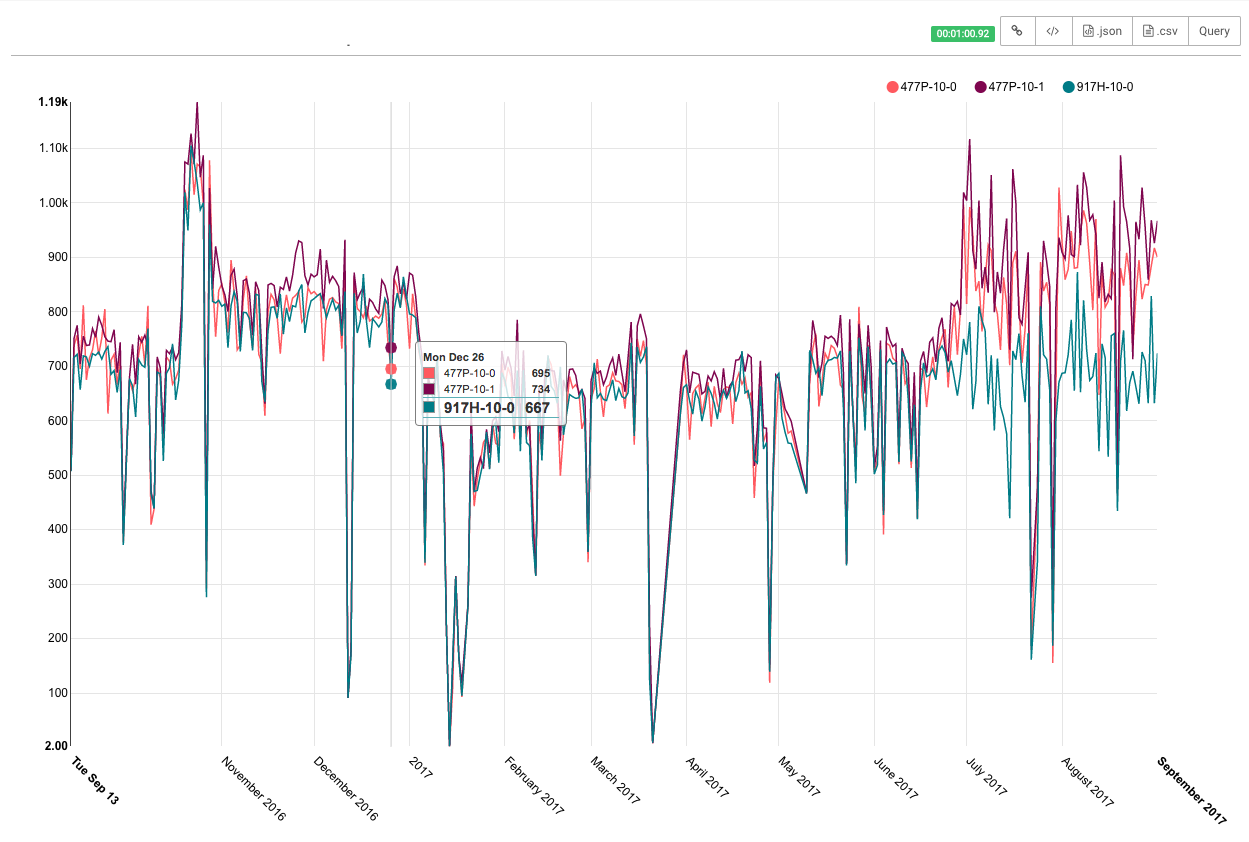
\includegraphics[width=0.8\linewidth]{qtd_data_per_day477p971h}
	\label{fig:qtd_data_per_day477p971h}
\end{figure}

\end{frame}
%------------------------------------------------
\begin{frame}
\frametitle{Exploração e visualização do conjunto de dados}
\begin{figure}[H]% H manda colocar exatamente nessa posição no texto (relativa aos parágrafos anterior e posterior)
	\centering
 	  \caption{Quantidade de dados enviados por ônibus / mês: viagens 477P-10-0, 477P-10-1 e 971H-10-0}
		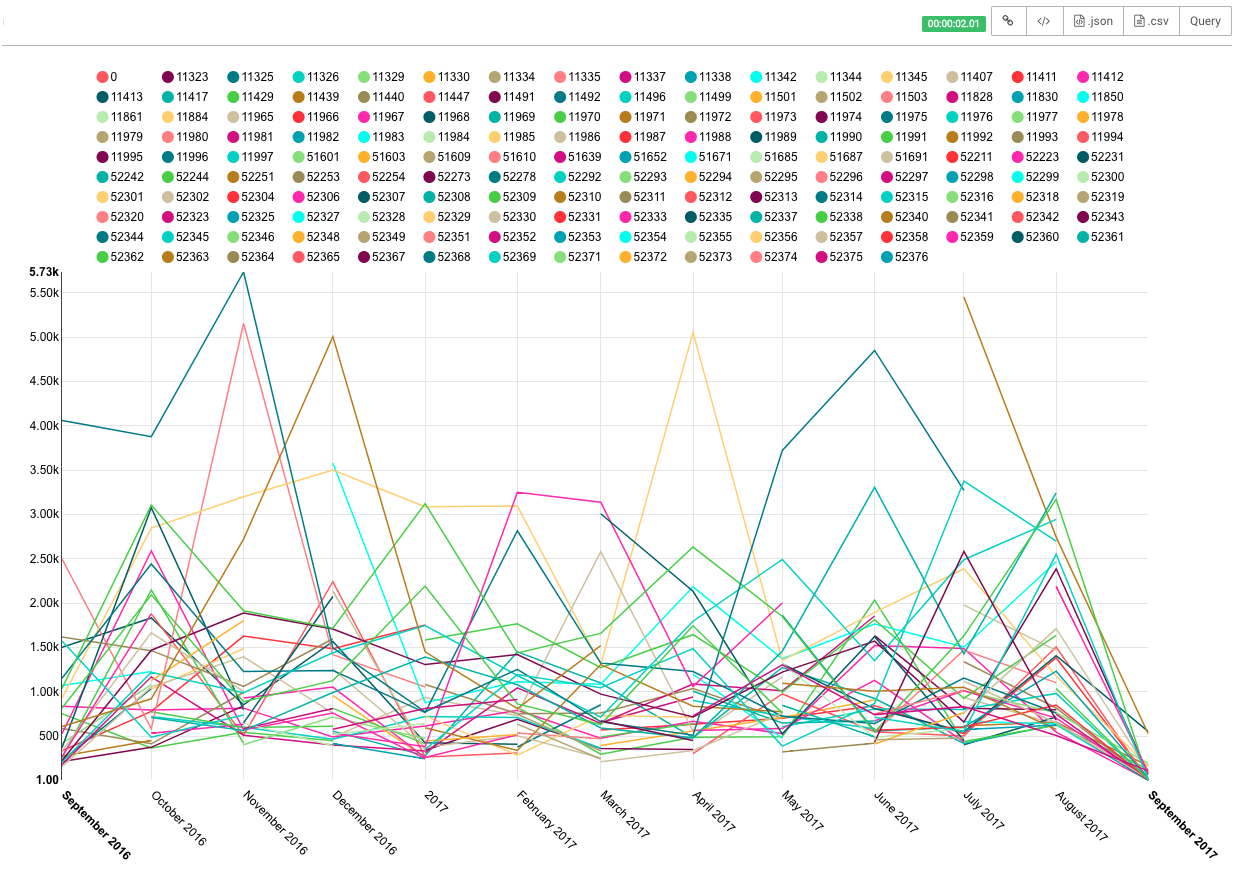
\includegraphics[width=0.8\linewidth]{qtd_data_per_bus_month_477p971h}
	\label{fig:qtd_data_per_bus_month_477p971h}
\end{figure}

\end{frame}
%------------------------------------------------
\begin{frame}
\frametitle{Exploração e visualização do conjunto de dados}
\begin{figure}[H]% H manda colocar exatamente nessa posição no texto (relativa aos parágrafos anterior e posterior)
	\centering
 	  \caption{Localizações de envio dos dados: viagens 477P-10-0, 477P-10-1 e 971H-10-0}
		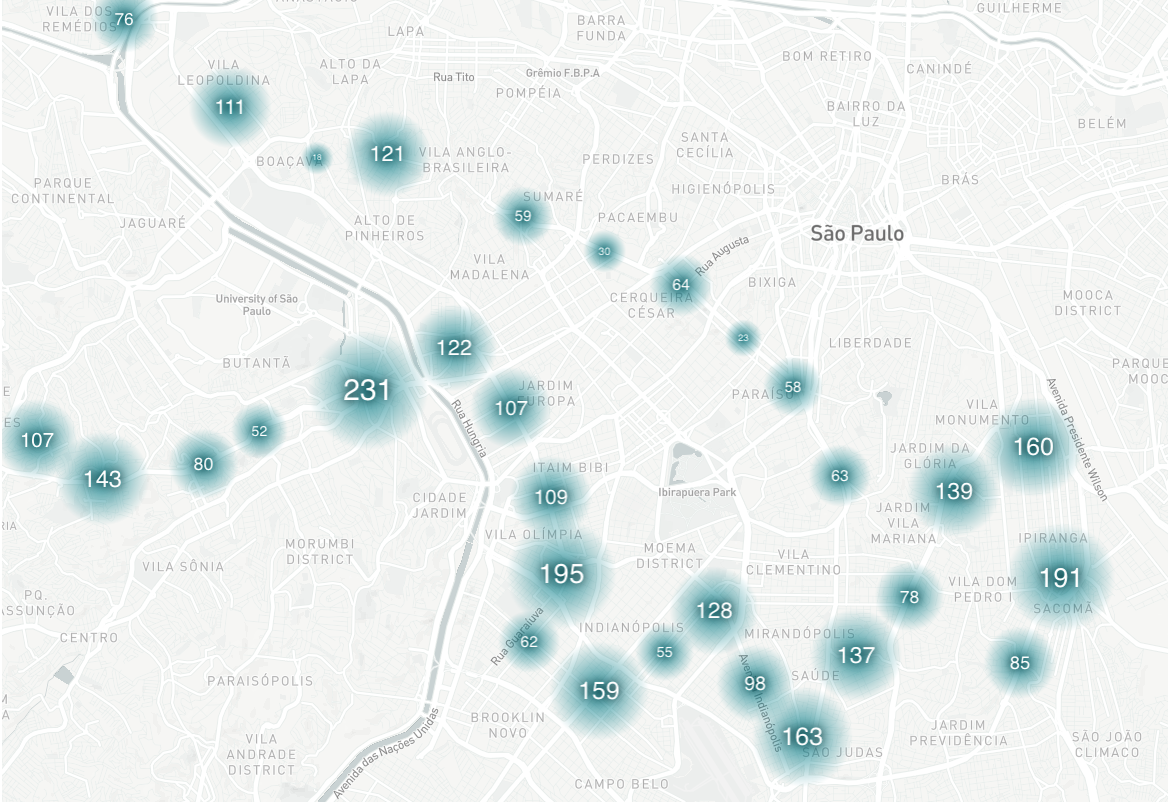
\includegraphics[width=0.7\linewidth]{map_477p971h}
	\label{fig:map_477p971h}
\end{figure}
\end{frame}
%------------------------------------------------
\subsection{Plano de trabalho}
\begin{frame}
\frametitle{Plano de trabalho}
\begin{table}[!htb]
  \centering
  \caption{Cronograma de atividades}
  \resizebox{\textwidth}{!}{%
    \begin{tabular}{cccccccccccccccccccc} \hline
    \multicolumn{2}{c}{Atividade } & \multicolumn{12}{c}{2017}                                                                     & \multicolumn{6}{c}{2018} \\ 
    Número & Descrição & 1     & 2     & 3     & 4     & 5     & 6     & 7     & 8     & 9     & 10    & 11    & 12    & 1     & 2     & 3     & 4     & 5     & 6 \\ \hline
    1     & Revisão bibliográfica & X     & X     & X     & X     & X     & X     &       &       &       &       &       &       &       &       &       &       &       &  \\
    2     & Desenvolvimento de protótipo &       &       & X     & X     & X     & X     &       &       &       &       &       &       &       &       &       &       &       &  \\
    3     & Construção do conjunto de dados &       &       &       &       &       &       & X     & X     & X     & X     & X     &       &       &       &       &       &       &  \\
    4     & Implementação da solução proposta &       &       &       &       &       &       &     &      &      &      &      & X     &   X    &  X     &   X    &  X   &   X   &  \\
    5     & Avaliação dos resultados &       &       &       &       &       &       &       &       &       &      &     &      &   X    &       &   X    &       &   X    &  \\
    6    & Escrita de artigo &       &       &       &       &       &       &       &       &       &       &      &       &       &   X    &   X    &       &       &  \\ 
    7     & Escrita da dissertação &       &       & X     & X     & X     & X     & X     & X     & X     & X     & X     & X     & X     & X     & X     & X     & X     & X \\
    \hline
    \end{tabular}%
    }
  \label{tab:schedule}%
\end{table}%
\end{frame}
%------------------------------------------------
\begin{frame}
\frametitle{Plano de trabalho}
\begin{itemize}
\item Implementação da solução proposta.
\begin{itemize}
\item Identificação dos eventos de exceção (pré-processamento, \textit{feature extraction} e \textit{feature selection} dos \textit{tweets} coletados).
\item Estudo dos algorítimos de classificação e implementação de um artefato de \textit{software} para classificação dos \textit{tweets} de acordo com seus respectivos eventos de exceção.
\item Correlação dos eventos de exceção com os dados AVL da SPTrans.
\end{itemize}
\item Avaliação dos resultados parciais obtidos durante e após o desenvolvimento da solução proposta.
\item Escrita de artigo para submissão em periódicos ou eventos da área.
\item Escrita da dissertação.
\end{itemize}
\end{frame}
%------------------------------------------------
\subsection{Contribuições esperadas}
\begin{frame}
\frametitle{Contribuições esperadas}
\begin{itemize}
\item Propor uma solução para o problema de caracterização de eventos de exceção e de seus respectivos impactos no sistema de transporte público por ônibus da cidade de São Paulo, por meio de \textit{tweets} e de dados históricos dos módulos AVL do SIM;
\item disponibilizar os os conjuntos de dados que foram construídos;
\item uma plataforma para que esses dados possam ser visualizados e explorados, de forma a contribuir com projetos e pesquisas futuras correlatas;
\item submissão de artigos com os resultados obtidos para veículos de disseminação de conhecimento científico nas áreas de: Análise de Redes Sociais, Sistemas de Transporte Inteligentes, Cidades Inteligentes.
\end{itemize}
\end{frame}
%------------------------------------------------
\subsection{Limitações e riscos à validade do estudo}
\begin{frame}
\frametitle{Limitações e riscos à validade do estudo}
\begin{itemize}
\item Processamento de \textit{tweets} em português brasileiro e oriundos das contas selecionadas, o que pode tornar a solução não generalista. 
\item É possível que sejam encontrados novos desafios que inviabilizem o uso de Expressão Regular para extração dos endereços dos \textit{tweets}.
\end{itemize}
\end{frame}
%------------------------------------------------
\end{document}